\documentclass{article}

% if you need to pass options to natbib, use, e.g.:
%     \PassOptionsToPackage{numbers, compress}{natbib}
% before loading neurips_2018

% ready for submission
% \usepackage{neurips_2018}

% to compile a preprint version, e.g., for submission to arXiv, add add the
% [preprint] option:
%     \usepackage[preprint]{neurips_2018}

% to compile a camera-ready version, add the [final] option, e.g.:
\usepackage[preprint]{neurips_2018}

% to avoid loading the natbib package, add option nonatbib:
%     \usepackage[nonatbib]{neurips_2018}

\usepackage[utf8]{inputenc} % allow utf-8 input
\usepackage[T1]{fontenc}    % use 8-bit T1 fonts
\usepackage{hyperref}       % hyperlinks
\usepackage{url}            % simple URL typesetting
\usepackage{booktabs}       % professional-quality tables
\usepackage{amsfonts}       % blackboard math symbols
\usepackage{nicefrac}       % compact symbols for 1/2, etc.
\usepackage{microtype}      % microtypography
\usepackage{graphicx}
\usepackage{amsmath}

\bibliographystyle{unsrtnat}

\title{MATH 189R HM Spring 2020 Final Report}

% The \author macro works with any number of authors. There are two commands
% used to separate the names and addresses of multiple authors: \And and \AND.
%
% Using \And between authors leaves it to LaTeX to determine where to break the
% lines. Using \AND forces a line break at that point. So, if LaTeX puts 3 of 4
% authors names on the first line, and the last on the second line, try using
% \AND instead of \And before the third author name.

\author{%
  Boyuan Chen \And
  Adam Guo \And
  Marcos Acosta \And
  Nathan Pappalardo
  % examples of more authors
  % \And
  % Coauthor \\
  % Affiliation \\
  % Address \\
  % \texttt{email} \\
  % \AND
  % Coauthor \\
  % Affiliation \\
  % Address \\
  % \texttt{email} \\
  % \And
  % Coauthor \\
  % Affiliation \\
  % Address \\
  % \texttt{email} \\
  % \And
  % Coauthor \\
  % Affiliation \\
  % Address \\
  % \texttt{email} \\
}

\begin{document}
% \nipsfinalcopy is no longer used

\maketitle

\begin{abstract}
  The utilization of facial shape as a vital element to improve the efficiency
  of facial recognition is a fresh topic for research. We propose a
  posterior-like combination of two predictions generated by a facial shape
  model and a CNN model, respectively. In such a way, the CNN network can save a
  lot of computations by only looking at the important facial areas, which are
  the eyes and the mouth.
\end{abstract}

%--------------------------------------

\section{Introduction}

The method of convolutional neural network is widely used in facial recognition
nowadays. Early since 2014, research teams have been trying to increase the
accuracy by designing more and more complicated structures. Nonetheless, with
each small amount of improvement in accuracy, the increase in computation is
tremendous. We want to find ways to improve the efficiency of the network while
not sacrificing too much of accuracy. 

One of the most challenging problem of facial recognition is rotation. While
humans can easily recognize a person even after they rotate a little bit, the
distribution of color on the pixels could become totally different. To solve
this problem, many teams have come up with ways to generate a frontal face
first, where they they apply normal CNN to. Nevertheless, the accuracy of
frontalization is always questionable, and those methods with high accuracy are
hard to train by themselves. 

We thus propose an easier way to utilize the extracted shape feature to
facilitate CNN recognition - a posterior combination. By training a model that
extracts facial shape and set the result as input to a clustering model, we can
get a prediction of each person P1, based on the shape alone. Then, combining
with the prediction P2, generated by CNN, we will have a reliable prediction
that takes into account both the face contour and the details on the face. Note
that since P2 does not have to cover the face contours, it can train on a much
smaller image and thus improve efficiency.

%--------------------------------------

\section{Datasets}

We used two datasets consisting of images of faces. The first is VGGFace2
(\cite{vggface2}), a set of over 3.3 million images of 9000+ people, captured
"in the wild" with natural poses, emotions, and lighting. We extracted roughly
500 images each of 10 celebrities, and aim to recognise which person any one of
these images belongs to. After we downloaded the dataset, we had to remove any
"impurities" in the dataset manually, including pictures with tilted faces,
incomplete/non-existing faces, or faces covered by hair or other objects, and
even pictures containing faces of a different person.

The second is the Head Pose Image Database from the Pointing'04 ICPR Workshop
(hereafter referred to as the Pointing dataset) (\cite{pointing}). This database
provides 15 sets of images, each of which contains 93 images of a single person
at different poses. We use this dataset to analyse facial rotations, as well as
to provide a set of clean, consistent images of frontal pose.

%--------------------------------------

\section{Extracting Face Shape Information}

Here we will mostly introduce our attempts on 2D face shape extraction by far.
It is proved to be insufficient in the final result, so we will move on to 3D
face shape construction in the summer.

\subsection{dlib}

Dlib for face detection uses a combination of HOG (Histogram of Oriented
Gradient) and Support Vector Machine (SVM). The dlib method of using HOG for
semi-rigid objects detection was first published in 2005, and refined for
multiple times since then (\cite{Kazemi2014OneMF}). A dlib HOG model is trained
through feeding in images with the items in interest having labeled boxes on the
surroundings. According to the publisher, the human face detector only took 6
seconds to train. In comparison, a Haar Cascade detector could take hours, even
days to train. In addition, dlib's structural SVM training algorithm is used in
the HOG trainer, efficiently reducing the amount of tedious sampling and
training data needed.

\subsection{Jaw Shape Vector (Rotation of dlib coordinates)}
\label{section:dlib_rotation}

Clustering facial images involves two major steps: rotating input images to face
the camera, and using a clustering algorithm to predict probabilities that an
image belongs to a person. We first discuss the image rotation process. 

We first fix the z-axis (vertical to the paper) rotation by normalizing the
coordinates to the center, and then rotating the dots via linear transformation
so that the center of the eyes form a line parallel to the x-axis. The scaling
of normalization is dependent on the length of the first dot. We set its
distance to the origin as 100 pixels, and all the other dots are multiplied by
the same scale. This procedure is described in the first row of Figure
\ref{fig:dlib_example}.

Then, we take the bigger half of the face and put it on the xy-plane. We rotate
the face around y-axis for an angle that is proportional to the ratio of areas
of the bigger half and the smaller half. This process is described in the second
row of Figure \ref{fig:dlib_example}.

Lastly, we project the rotated bigger-half back to the xy-plane. Then, mirror it
to the other side to get a full face. Eventually, we find the center of the face
and take the lengths of the 17 shoots to form a vector that represents this face
shape.

\begin{figure}[ht]
  \centering
  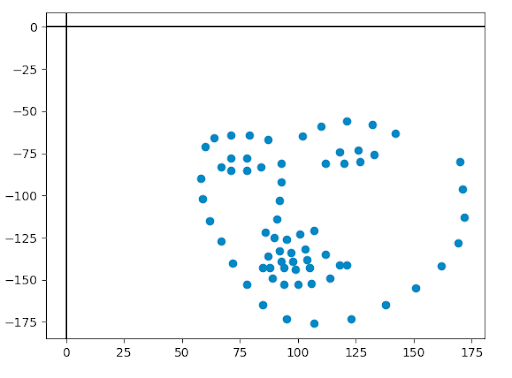
\includegraphics[width=5cm]{images/dots_transformation/dots1.png}
  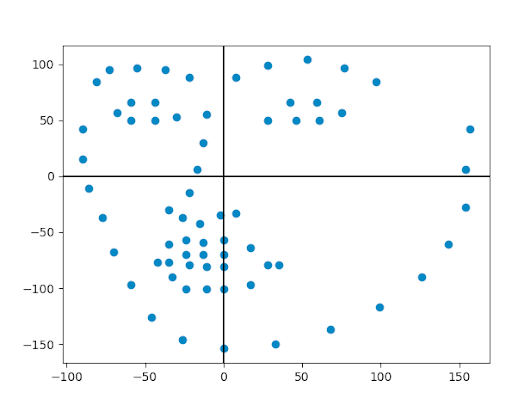
\includegraphics[width=5cm]{images/dots_transformation/dots2.png}
  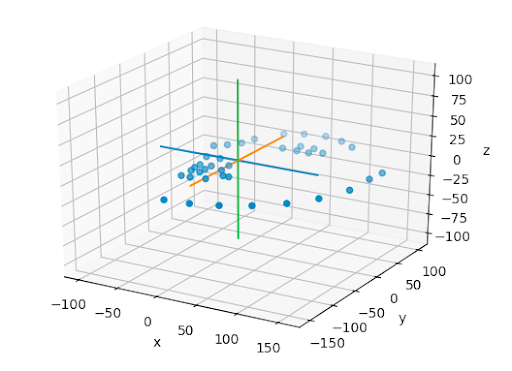
\includegraphics[width=5.5cm]{images/dots_transformation/dots3.png}
  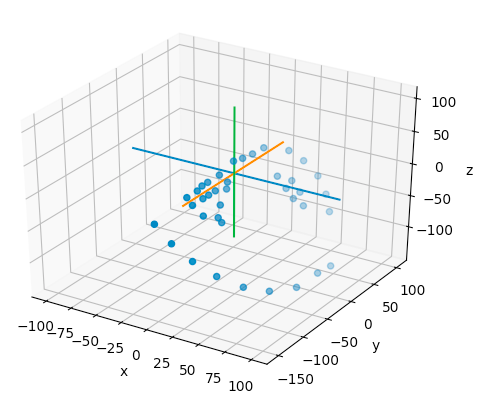
\includegraphics[width=5cm]{images/dots_transformation/dots4.png}
  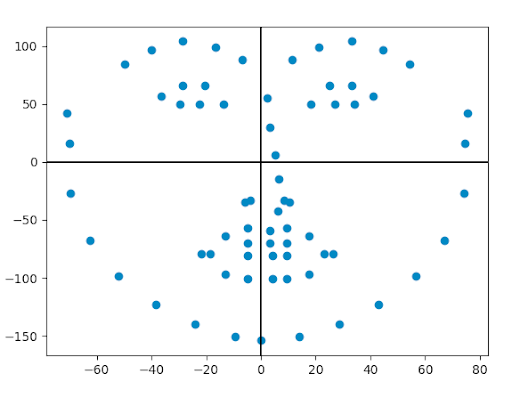
\includegraphics[width=5cm]{images/dots_transformation/dots5.png}
  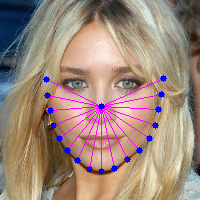
\includegraphics[width=4cm]{images/dots_transformation/dots6.png}
  \caption{Example of facial shape clusters among 14 people}
  \label{fig:dlib_example}
\end{figure}

\subsection{Next Step: 3D Face Shape Reconstruction}
\label{section:3D_reconstruction}

As will be discussed later, the result is not satisfactory because the frontal
shape generating function is naive. We will focus on searching for existing
methods in generating 3D face shapes. Such is a hot topic in recent years, and
there are good models such as Position Map Regression Network
(\cite{feng2018joint}, GANFIT(\cite{ganfit}), Unsupervised Training for 3D
Morphable Model Regression (\cite{genova2018unsupervised}), etc. The ideal
method is one that takes multiple inputs from the same person of different
angles, so that the 3D-reconstructed mesh should be more accurate.

%--------------------------------------

\section{Clustering facial vectors}

For this section, our goal is to obtain geometric information from facial images
to compute a posterior based on facial shape, which can be multiplied to priors
generated by facial features to yield a final prediction of who the given face
belongs to. Given a sample of facial images, different types of facial shapes
roughly emerge. That is, we can categorise people by how similar their facial
shapes are (figure \ref{fig:cluster_example}). Hence, we used unsupervised
probabilistic clustering to learn clusters of face shapes from some input data
and compute a probability that any given face belongs to some cluster. This
probability gives an effective likelihood that an input face matches some person
with a face shape in that cluster, which we can use as our posterior.

\begin{figure}[ht]
  \centering
  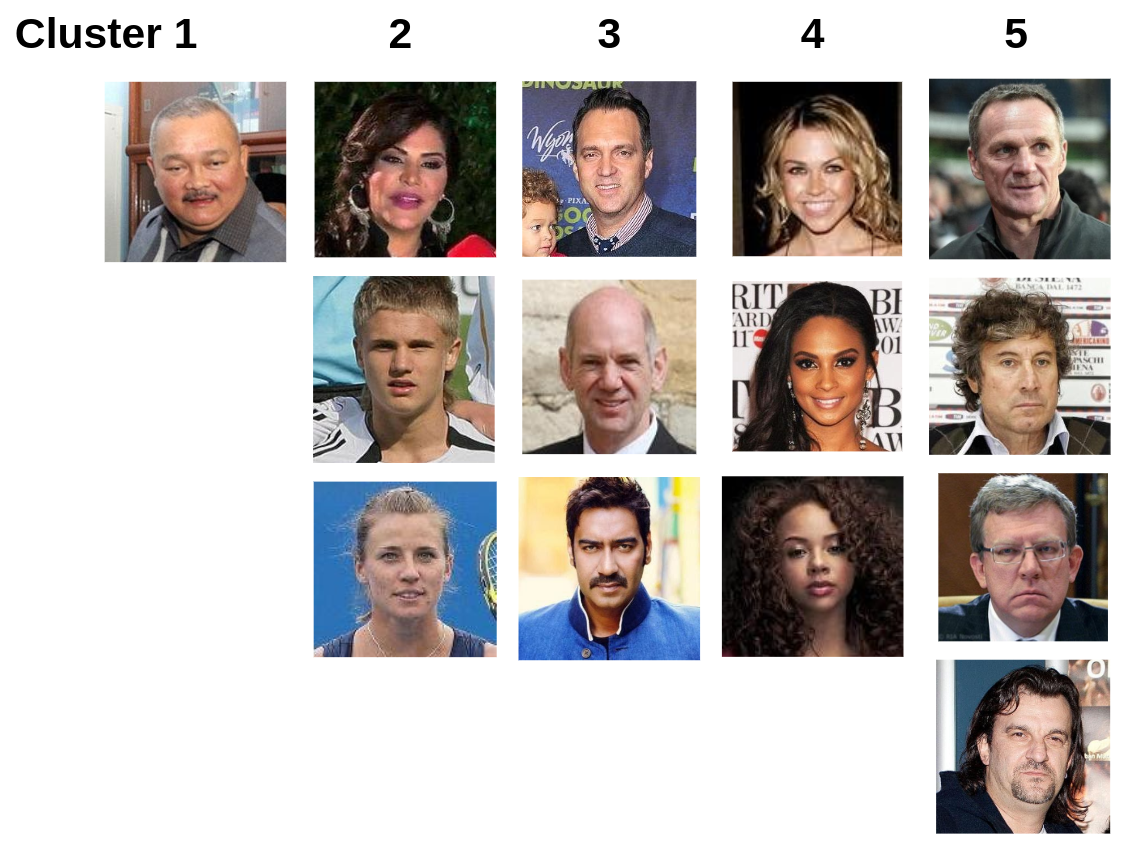
\includegraphics[width=10cm]{images/cluster_example.png}
  \caption{Example of facial shape clusters among 14 people}
  \label{fig:cluster_example}
\end{figure}

We chose to use a Gaussian mixture model (GMM), which consists of a weighted sum
of $K$ multivariate normal distributions (\cite{murphy}):

\[p(x_i : \theta) = \sum_{k=1}^K \pi_k \mathcal{N}(x_i : \mu_k, \Sigma_k)\]

The parameters of each Gaussian and their associated weights can be fitted using
expectation maximisation, giving us probabilistic clusters for facial shapes.
The Python package \texttt{scikit-learn} includes a native GMM model trainer,
\texttt{GaussianMixture}, which we used to train on the 17-dimensional vectors
that represent the facial shape of each image.

\subsection{Using GMM clustering for recognition}
\label{section:cluster_initial}

Our initial approach to clustering faces was to determine whether or not many
frontal images of a particular person were enough to discern a distinct shape
cluster corresponding to their real face. We manually sorted through images of 5
celebrities, picked images that were frontal-facing (centered along the x, y,
and z axes), computed their shape vectors, and clustered them using GMM ($K =
5$).

The 3-dimensional PCA visualisation (figure \ref{fig:pca_cluster}) shows that
the clustering of the original data is not well-defined. The GMM fitted 5 naive
clusters by effectively slicing the data into 5 chunks, yielding an accuracy of
25\% (around random) when predicting which person an image corresponded to. This
test confirmed that there is significant variability in the shape vectors of
each person depending on minute changes in the angle at which the image is
taken. Manually selecting many frontal images of a single person is insufficient
in eliminating angle variations.

\begin{figure}[ht]
  \centering
  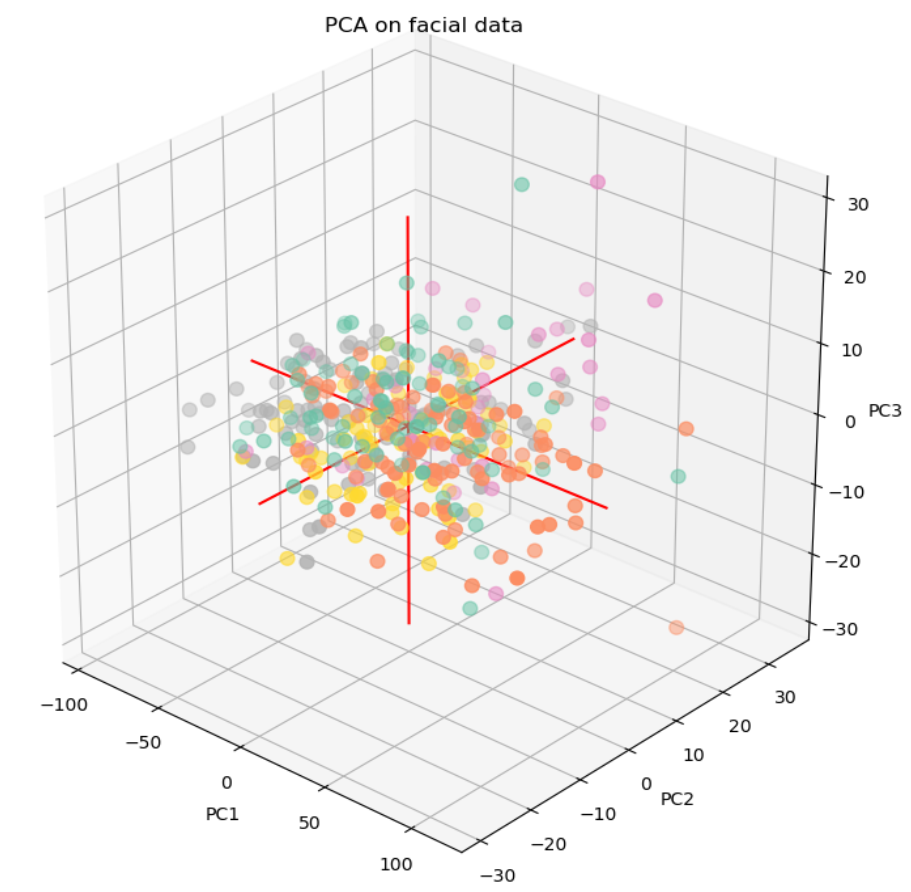
\includegraphics[width=6cm]{images/pca_1.png}
  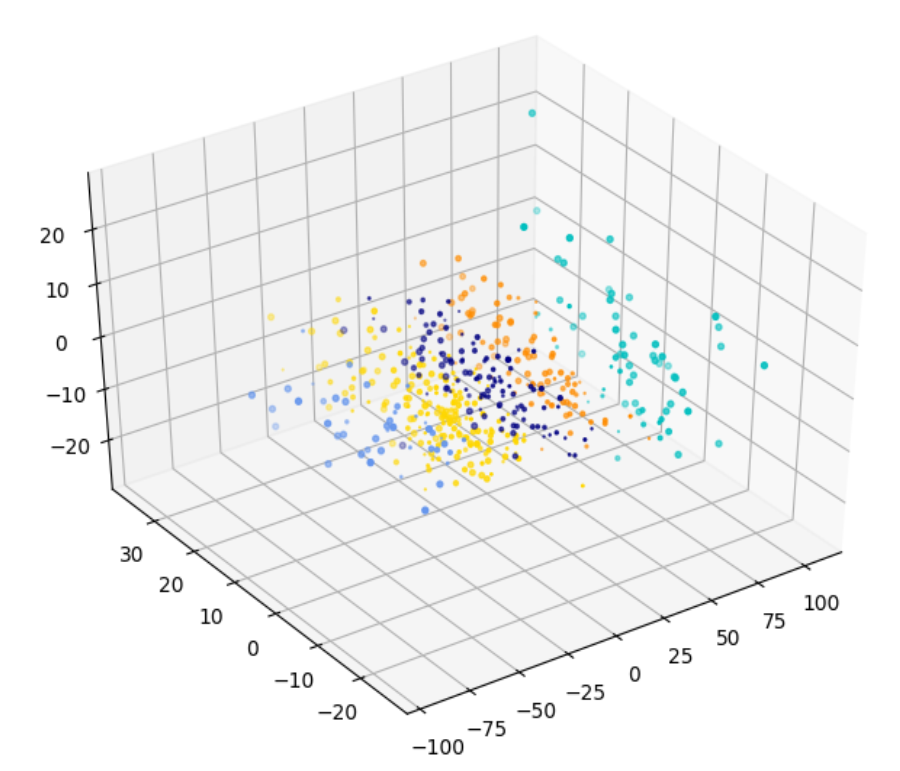
\includegraphics[width=6cm]{images/cluster_1.png}
  \caption{Original and clustered data, shown on 3D PCA of facial vectors}
  \label{fig:pca_cluster}
\end{figure}

\subsection{Using GMM clustering on broad-based sample}

The above clustering attempt revealed the inadequacy of geometric information in
predicting the identity of an image. This led us to an alternate approach for
analysing geometric facial information: instead of training a clustering model
on the faces we wish to recognise, we decided to train a model on a broad-based
sample of the general human population. The intuition is that by recognising
latent face types in the broader population, the model can probabilistically
group people in the test database. Then, given an image to infer on, the model
can evaluate the likelihood that the image belongs to each cluster, and thereby
the likelihood that the image belongs to each person in the test database.

The Pointing dataset provides images of many individuals taken in
a standard frontal pose. We trained the same Gaussian mixture model as above on
the new set of data, producing the clusters shown in figure
\ref{fig:broad_sample}. Note that the overall structure is similar to figure
\ref{fig:pca_cluster}, the difference being that since in this case each vector
corresponds to a unique person, we expect a diffusely scattered plot with evenly
divided clusters, rather than obvious clusters corresponding to multiple images
of a single person.

\begin{figure}[ht]
  \centering
  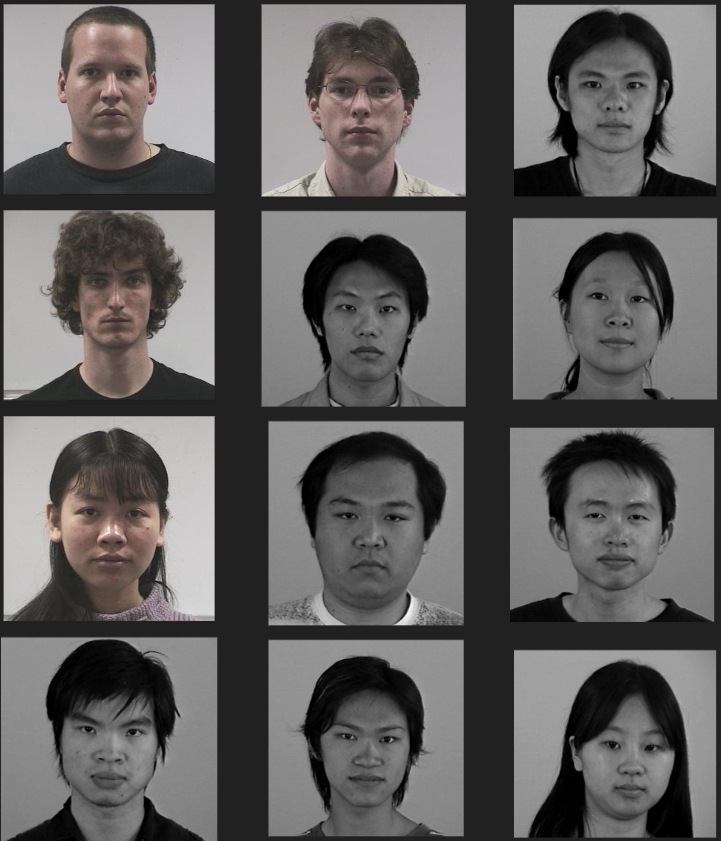
\includegraphics[width=5cm]{images/frontal_sample.png}
  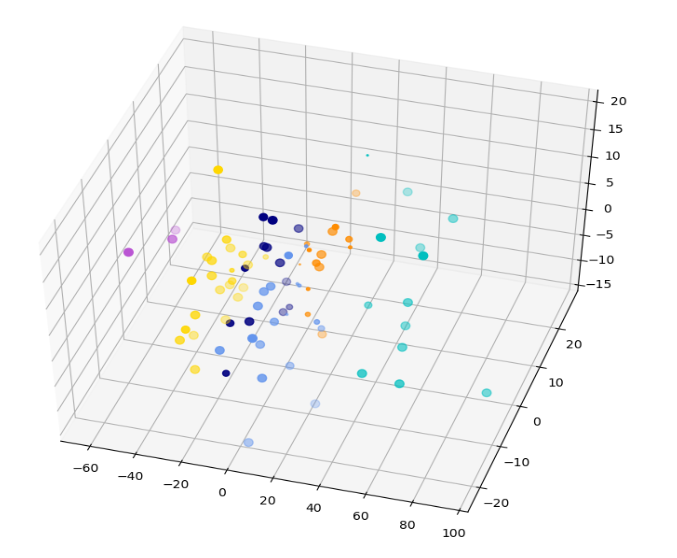
\includegraphics[width=8cm]{images/broad_pca.png}
  \caption{Left: sample of Pointing dataset, right: PCA 3D
  projection of facial vectors}
  \label{fig:broad_sample}
\end{figure}

\subsection{Computing posterior}

Using the trained Gaussian mixture model, we now compute the posterior: the
probability that an input face belongs to any person in the dataset. Note that
we are aiming to recognise individual celebrites in VGGFace2, not individuals in
the Pointing dataset.

Suppose we have a dataset of $n$ people, where the $i$th person has $m_i$
images. Let $\mathbf{v}^{(i)}_j \in \mathbb{R}^{17}$ be the vector generated by
\texttt{dlib} that represents the jawline of the $j$th image corresponding to
person $i$. Let $k$ be the number of components (i.e. clusters) in the GMM. Let
$Z : \mathbb{R}^{17} \rightarrow \mathbb{R}^k$ be a function where
$Z(\mathbf{x})$ is the probability vector returned by the GMM given input vector
$\mathbf{x}$.

We construct a matrix $M \in \textsf{\textbf{M}}_{n \times k}$ as follows:

\[M = \begin{bmatrix}
  \frac{1}{m_1} \sum_{j=1}^{m_1} Z(\mathbf{v}_j^{(1)})^T \\
  \frac{1}{m_2} \sum_{j=1}^{m_2} Z(\mathbf{v}_j^{(2)})^T \\
  \vdots \\
  \frac{1}{m_n} \sum_{j=1}^{m_n} Z(\mathbf{v}_j^{(n)})^T
\end{bmatrix}\]

The $(i, j)$ element of $M$ is the likelihood that person $i$ belongs to cluster
$j$, which we interpret as the weight of cluster $j$ in predicting person $i$.
We divide by the number of images that person has to prevent biasing towards
people with more images in the dataset. Given an input vector $\mathbf{x} \in
\mathbb{R}^{17}$ we wish to predict, we use the model to infer $\mathbf{p} =
M(\mathbf{x}) \in \mathbb{R}^k$, then compute

\[\mathbf{y} = M\mathbf{p} \in \mathbb{R}^n\]

Normalising $\mathbf{y}$ such that the entries sum up to 1, we have the
posterior:

\[\tilde{\mathbf{y}} = \frac{1}{\sum_{i=1}^n y_i} \mathbf{y}\]

$\tilde{\mathbf{y}}$ gives the probability that the input $\mathbf{x}$ is an
image of each of the $n$ people. Specifically, $\tilde{y}_i$ gives the
probability that the input is an image of the $i$th person.

\subsection{Result}

Running the full posterior computation pipeline, we experienced more issues
related to noise in the facial vectors. We trained a GMM $M_f$ on the Pointing
dataset of frontal images, using $k = 6$ components, and fed celebrity images
from the VGGFace2 dataset to predict on. However, regardless of which image is
given as input, $M_f$ always returned a prediction of $\begin{bmatrix} 0 & 0 & 0
& 0 & 1.0 & 0 \end{bmatrix}$. The model is essentially 100\% confident that
every input image belongs to the same cluster, with zero probability of
belonging to any other cluster. As a result, the posterior computation yielded a
uniform probability that any input image belongs to each person.

As a sanity check, we repeated the process using another GMM $M_c$, trained on
VGGFace2 itself (akin to Section \ref{section:cluster_initial}). While the
results this time made more sense and did not predict that every image belonged
to the same cluster, this approach suffered from the same problems faced in
Section \ref{section:cluster_initial}, which were that the predictions were very
inaccurate (~25\%).

Our posterior computation method is quite straightforward and seemed to be
working. Instead, the problem lies with the results predicted by the GMM.
Examining the reconstructed frontal facial vectors that were generated in
Section \ref{section:dlib_rotation}, we concluded that the coordinate
transformation process distorts each face in a consistent manner by stretching
each face horizontally and also creating a perfectly symmetrical face across the
vertical axis. While these differences were not apparent to human viewers, they
could very well have been perceptible and consistent enough for $M_f$, which was
originally trained on non-transformed faces, to discern a common structure and
assign them all to the same cluster, regardless of what the original face was.

This suggests that our clustering approach does not go well with our coordinate
transformation process. To compute a usable posterior, we need to re-evaluate
our strategy these two steps of the pipeline.

%--------------------------------------

\section{Future steps}

Though our result is far from satisfying, we hold faith in the general structure
and are quite certain about our next steps. The clustering method appears
functional and thus should be largely kept. However, there are some important
changes that can be made. First, the clustering approach assumes that there are
discrete categories that faces can be grouped into. Our data reveals that this
is not really true: faces are largely continuous structures, and while as humans
we can say that some faces have distinct shapes, there is no clear boundary
between these categories. Hence, instead of a clustering algorithm, we can move
to computing weights based on the raw distances between vectors (with an
appropriate distance function), allowing us to bypass the problems we have had
with Gaussian mixture models.

Generating face shape vectors has significant room for improvement. As mentioned
in Section \ref{section:3D_reconstruction}, we will search for more recent
approaches in 3D face shape construction. The most popular models take only 1
image as the input. Though good enough on its own standard, we aim to find ways
to incorporate multiple images of one person's face to generate a more accurate
3D mesh.

Furthermore, recent advances have also provided a better possibility for
generating the second possibility via CNN. Several papers have offered ways to
generate frontal face images via GAN. Jian Zhao finished the whole pipeline of
using the frontal face generated by GAN for CNN facial recognition, and is
proved to have good result (\cite{Zhao2018CVPR}). We would like to use these
works as methods to generate the second probability in the posterior.

\newpage

\bibliography{citations.bib}

\end{document}